A scientific experiment is carried out in order to obtain empirical data and to test the hypotheses put forward. To distinguish it from an observation, independent variables are manipulated in an experiment under controlled conditions. The independent variable in turn influences a dependent variable. In the next step, the independent variable is deliberately manipulated and the dependent variable reacts to this event\footcite{genau_experiment_2018}.
For our research, a laboratory experiment comes into question, as we create an artificial environment in which we can control all variables well. Due to the artificial environment we have created, assumptions can be made, but the results cannot be generalized with complete certainty\footcite{genau_experiment_2018}.
In this chapter we describe our experimental design for our explanatory research. 
For our experimental design, we orientated on four key steps that help us to perform a theory based and structured experiment. The four key steps are:\footcite{bevans_guide_2019}\newline
\begin{itemize}
    \item Defining our variables
    \item Writing our hypothesis
    \item Designing our experimental treatments
    \item Measure our dependent variable
\end{itemize}

\textbf{Defining our Variables} \newline

\begin{figure}[H]
    \centering
    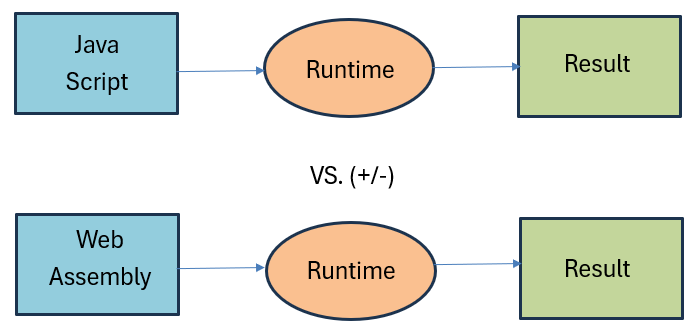
\includegraphics[width=1\textwidth]{Comparison Design.PNG}
    \caption{Comparison Design, Source: Own depiction}
	\label{fig:compdesign}
\end{figure}

In that case our question is, if and how the runtime can be affected by whether using JavaScript or using WASM for different computationally intensive operations. The key independant variables are „JavaScript“ and „WASM“. The key dependant variable is „Runtime“. Abb.X is further called „Fixed testing part“.
To specify different input operations, we will show them in the following figures, while there is the fixed test part as shown above and the "operation part" for the different test operations, which define the input given to each, JavaScript and WASM within the fixed test part.

\begin{figure}[H]
    \centering
    \caption{Advanced Comparison Design, Source: Own depiction}
	\label{fig:comparison}
    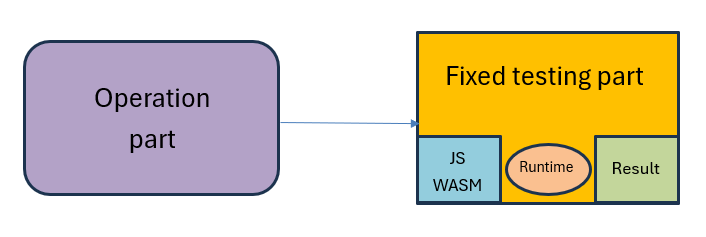
\includegraphics[width=1\textwidth]{Comparison 2.PNG}
\end{figure}

\begin{table}[H]
    \centering
    \caption{Differenciation of dependant and independant variables, Source: Own depiction}
	\label{fig:variables}
    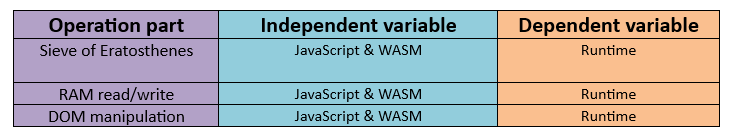
\includegraphics[width=1\textwidth]{Table variables.PNG}
\end{table}

The first operation part is about the Sieve of Eratosthenes. The code is written in both, JavaScript and for WASM with Rust. Both programming languages are the independent variables, which are effecting the dependent variable runtime directly.
The third operation part is about DOM manipulation. Here, the independent variables are JavaScript and WASM. The dependent variable, affected be the independent variables JavaScript and WASM, is runtime.

\textbf{Writing our hypothesis} \newline
Now that we have defined our testing variables, we can put our hypothesis for each operation part in position\footcite{bevans_guide_2019}.

\begin{table}[H]
    \centering
    \caption{Definition of hypothesis for each operation part, Source: Own depiction}
	\label{fig:hypothesis}
    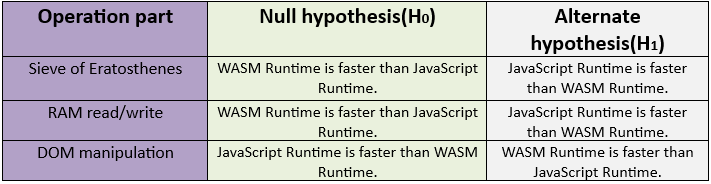
\includegraphics[width=1\textwidth]{Table hypothesis.PNG}
\end{table}

With the execution of the Sieve of Eratosthenes algorithm it is assumed that WASM has a faster Runtime than JavaScript.
For RAM read and write operations it is assumed that WASM has a faster runtime than JavaScript.
For the third hypothesis it is assumed that JavaScript has a faster Runtime than WASM for DOM manipulation.

\textbf{Design our experimental treatments} \newline
In order to carry out a realistic test experiment, it is necessary to make various changes to the variables. This allows a wide variety of conditions to be tested and the resulting findings to be recorded. Different variables ensure that the experiment is as valid as possible\footcite{bevans_guide_2019}.
In our case we simply change the operation part to manipulate our independant variables. By changing this, JavaScript and WASM can be compared on different ways in different use cases, so that we can collect as many results as possible and useful for our comparison and research goal.

\textbf{Measure our dependent variable} \newline
In the end, we will collect all the data from the testing cases (operation part) and measure them, to answer our hypothesis.
